\section{Modern CPU Vulnerabilities}
\frame{\sectionpage}

\begin{frame}{GoFetch}{Boru Chen et al. of University of Illinois Urbana-Champlain}
    \label{gofetch} 
    \begin{itemize}
        \item \href{https://www.usenix.org/system/files/usenixsecurity24-chen-boru.pdf}{\color{pink}GoFetch} is a side-channel attack against Apple's Data Memory Prefetcher (DMP).
        \item The DMP looks at data in registers entering the pipeline, if a value \textit{looks} like a pointer, the DMP preemptively loads its cache line. 
        \item This can artificially introduce timing issues in cryptographic algorithms, since a known ciphertext attack can accelerate rounds of constant time algorithms. 
    \end{itemize}
    \begin{figure}
            \centering
            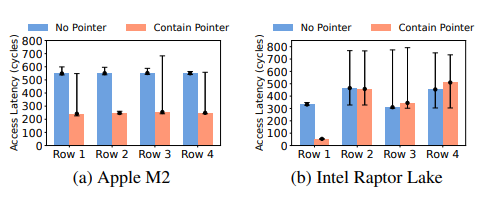
\includegraphics[width=0.51\textwidth]{images/gofetch_graphic.png}
            \caption{The timing differences of cache lines which contain pointers as a result of the DMP.}
            \label{fig:gofetch-dmp-timing}
    \end{figure}
    \note{
        \begin{itemize}
            \item Looks like a pointer, talks like a pointer...
            \item The Apple M1 chip's Firestorm core has a 128KB L1 cache, with 8 16KB cache sets with 64 byte cache lines.
            \item In the paper, the authors were able to break RSA and Diffie-Hellman within a few hours. They also break Kyber and other post-quantum algorithms.
        \end{itemize}
    }
\end{frame}

\begin{frame}{Downfall}{Daniel Moghimi of University of California San Diego}
    \label{downfall} The \href{https://downfall.page/media/downfall.pdf}{\color{pink}Downfall} attack leverages the \textit{gather} instruction on the x86 architecture to leak data from a common core. In operates in four steps,
    \begin{columns}
        \begin{column}{0.45\textwidth}
            \begin{enumerate}
                \item Execute a cache miss to prepare state
                \item Load data from an uncacheable address, such that \textit{gather} gets interrupted
                \item Speculatively store the data from \textit{gather} back into the cache
                \item Side-channel the (leaked!) data from the cache
            \end{enumerate}
        \end{column}
        \begin{column}{0.55\textwidth}
            \usemintedstyle{vim}
            \inputminted{c}{code/downfall.c}
        \end{column}
    \end{columns}
    \note{
        \begin{itemize}
            \item Note that step (3) never executes! The processor speculates the code and fails to properly cleanup for speculation.
            \item There are three distinct "vulnerable" sequences here demonstrated in the paper.
                \begin{enumerate}
                    \item In case 1, the memcpy is properly sanitized. However, the attacker can leak from such a gadget if using vulnerable instructions because the vectored instructions will out-of-bounds read themselves.
                    \item Case 2 is the trickiest, the memory copy always executes, but the length can be 0. As it turns out, this is also exploitable. 
                    \item Case 3 is a genuine software bug, with insufficient checks on the attacker controlled "index" field. While tihs may be an unexploitable bug (i.e. local never makes it back to the attacker), downfall can return that back to the attacker. 
                \end{enumerate}
        \end{itemize}
    }
\end{frame}

\begin{frame}{A Security RISC}{Lukas Gerlach et al. of CISPA Helmholtz Center for Information Security}
    \label{a-security-risc} \href{https://publications.cispa.saarland/3924/1/security_risc.pdf}{\color{pink}A Security RISC}, published in 2023, shows microarchitectural vulnerabilities on COTS RISC-V dev boards. It demonstrated three distinct attacks,
    \begin{enumerate}
        \item \textit{Cache+Time}, which exploits the branch predictor and the \textit{fence.i} instruction.
        \item \textit{Flush+Fault}, which jumps to arbitrary code to determine whether the victim ran it.
        \item \textit{CycleDrift} exploits a quirk where the CPU allow access to \textit{mcycle} and \textit{minstret}, counting clock cycles and instructions retired respectively. This allows attackers to infer execution.
    \end{enumerate}
    \begin{figure}
        \centering
        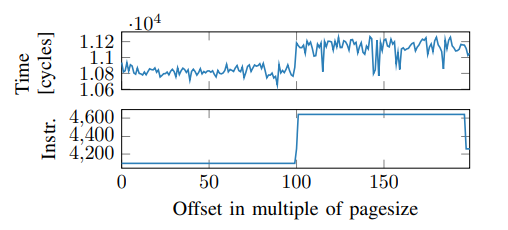
\includegraphics[width=0.4\textwidth]{images/asecurity_risc_graphic.png}
        \caption{Memory access times measured via CycleDrift during intentional page faults.}
        \label{fig:asecurity-risc-fault}
    \end{figure}
    \note{
        \begin{itemize}
            \item Before this paper released, the RISC-V ISA manual actually suggested that a naive implementation of fence.i instruction is to just flush the instruction cache. This was a bad suggestion.
            \item Similar specification level flaws for mcycle and minstret. 
            \item In case 1, \textit{fence.i} flushes the entire instruction cache, and the branch predictor will speculatively prefetch addresses, which can allow an attacker to populate a single cache line and measure victim repsonse time. 
            \item The distinct line within the graphic shows whether the memory was mapped or not, since it inherently contains the execution path of the kernel.
            \item In case 2, the instruction cache is executed, then the victim process runs a bit. If you then jump to an arbitrary address you can measure a timing difference based on a cache miss. 
        \end{itemize}
    }
\end{frame}